\documentclass[../differential_geometry.tex]{subfiles}
\begin{document}
\section{Aula 14 - Bônus}
\subsection{Motivações}
\begin{itemize}
	\item Aplicações Conformes.
\end{itemize}
\subsection{Aplicações Conformes}
\begin{def*}
	Uma aplicação \(f:S\rightarrow \tilde{S}\) é uma \textbf{aplicação conforme} se é um difeomorfismo e existe \(\lambda :S\rightarrow \mathbb{R}^+\) tal que
	\[
		\langle \mathrm{d}f_{p}(w_1), \mathrm{d}f_p(w_2) \rangle = \lambda (p) \langle w_1, w_2 \rangle, \quad \forall w_1, w_2\in T_{p}S,\; p\in S.
	\]
	Se, para todo p em S, existir uma parametrização local \(\underline{x}:U\rightarrow S\) com \(p\in \underline{x}(U)\) tal que \(f:\underline{x}(U)\rightarrow f(\underline{x}(U))\) é uma aplicação conforme, diremos que f é uma \textbf{aplicação conforme local}. \(\square\)
\end{def*}
Já pela definição, podemos inferir que aplicações conformes preservam ângulos; de fato, seja \(\theta \) o ângulo entre duas curvas \(\alpha \) e \(\beta \) em S com \(\alpha (0) = \beta (0) = p\); então,
\[
	\cos^{}{\theta } = \frac{\langle \alpha', \beta' \rangle}{\Vert \alpha' \Vert\Vert \beta' \Vert},
\]
enquanto que o ângulo \(\tilde{\theta }\) entre \(f\circ \alpha \) e \(f\circ \beta \) satisfaz
\[
	\cos^{}{\tilde{\theta }} = \frac{\langle (f\circ \alpha )', (f\circ \beta )'  \rangle}{\Vert (f\circ \alpha )' \Vert \Vert (f\circ \beta )' \Vert}.
\]
Porém, \((f\circ \alpha )' = \mathrm{d}f_{p}(\alpha ')\), tanto para \(\alpha \) quanto para \(\beta \), tal que
\begin{align*}
	\cos^{}{\tilde{\theta} } = \frac{\langle \mathrm{d}f_{p}(\alpha '), \mathrm{d}f_p(\beta ') \rangle}{\Vert \mathrm{d}f_p(\alpha ') \Vert\Vert \mathrm{d}f_p(\beta ') \Vert} & = \frac{\lambda \langle \alpha ',\beta '  \rangle}{\sqrt[]{\lambda }\Vert \alpha ' \Vert \sqrt[]{\lambda }\Vert \beta ' \Vert} \\
	                                                                                                                                                                           & = \frac{\langle \alpha ', \beta ' \rangle}{\Vert \alpha  \Vert\Vert \beta  \Vert}                                              \\
	                                                                                                                                                                           & = \cos^{}{\theta }.
\end{align*}
\begin{figure}[H]
	\begin{center}
		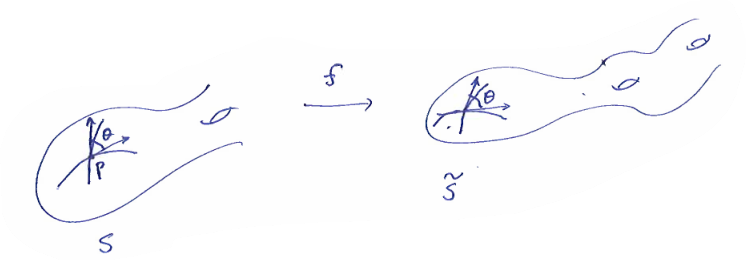
\includegraphics[height=\textheight, width=\textwidth, keepaspectratio]{./Images/conform_application_14.png}
	\end{center}
\end{figure}
\begin{tcolorbox}[
		skin=enhanced,
		title=Observação,
		fonttitle=\bfseries,
		colframe=black,
		colbacktitle=cyan!75!white,
		colback=cyan!15,
		colbacklower=black,
		coltitle=black,
		drop fuzzy shadow,
		%drop large lifted shadow
	]
	As isometrias são aplicações conformes com \(\lambda (p)\equiv 1\)!
\end{tcolorbox}

\begin{exr}
	Mostre que duas esferas com raios distintos são conformes, e que o plano e a esfera são localmente conformes.
\end{exr}
\begin{prop*}
	Seja \(\underline{x}:U\rightarrow S\) uma parametrização local de S. A aplicação \(f:S\rightarrow \tilde{S}\) é conforme em \(\underline{x}(U)\) se, e somente se, existe \(\lambda :U\rightarrow \mathbb{R}^{+}\) satisfazendo
	\[
		\langle f_u, f_u \rangle = \lambda E, \quad \langle f_u, f_v \rangle = \lambda f \quad\&\quad \langle f_v, f_v \rangle = \lambda G.
	\]
\end{prop*}
\begin{exr}
	Demonstre a proposição acima.
\end{exr}
\begin{prop*}
	Uma aplicação \(f:\underline{x}(U)\rightarrow \underline{\tilde{x}}(U)\) é conforme se, e somente se, existe \(\lambda :\underline{x}(U)\rightarrow \mathbb{R}^{+}\) tal que
	\[
		\tilde{E} = \lambda E, \quad \tilde{F} = \lambda F, \tilde{G} = \lambda G.
	\]
	\begin{figure}[H]
		\begin{center}
			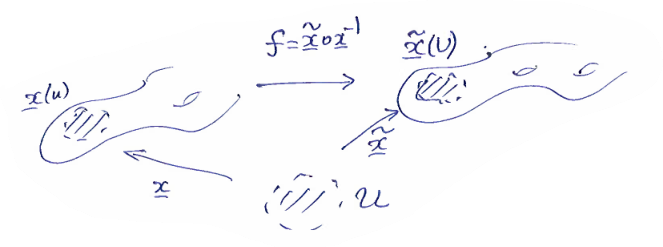
\includegraphics[height=\textheight, width=\textwidth, keepaspectratio]{./Images/scalar_characterization_14.png}
		\end{center}
	\end{figure}
\end{prop*}

\begin{example}[Conformidade da Catenoide com a Esfera]
	A aplicação de GAuss da Catenóide S é um exemplo de aplicação conforme! De fato, seja
	\begin{align*}
		\underline{x}: & (0, 2\pi )\times \mathbb{R}\rightarrow S                                                   \\
		               & (u, v)\longmapsto \underline{x}(u, v) = (\cosh^{}{v}\cos^{}{u}, \sinh^{}{v}\sin^{}{u}, v),
	\end{align*}
	de modo que
	\[
		E = G = \cosh^{2}{v}, \quad F = 0.
	\]
	Como já vimos,
	\[
		N = \frac{\underline{x}_{u} \times \underline{x}_{v}}{\Vert \underline{x}_u \times \underline{x}_v \Vert} = \frac{1}{\cosh^{}{v}}(\cos^{}{u}, \sin^{}{u}, -\sinh^{}{v}),
	\]
	donde temos
	\[
		\langle N_u, N_u  \rangle = \frac{1}{\cosh^{2}{v}}, \quad \langle N_u, N_v \rangle = 0 \quad\&\quad \langle N_v, N_v \rangle = \frac{1}{\cosh^{2}{v}}.
	\]
	Logo,
	\[
		\langle N_u, N_u \rangle = \lambda E, \quad \langle N_u, N_v \rangle = 0 \quad\&\quad \langle N_v, N_u \rangle = \lambda G,
	\]
	onde \(\lambda = \frac{1}{\cosh^{4}{v}}.\)

	Daí, como N é um difeomorfismo (exercício), segue a conformidade de N.
	\begin{figure}[H]
		\begin{center}
			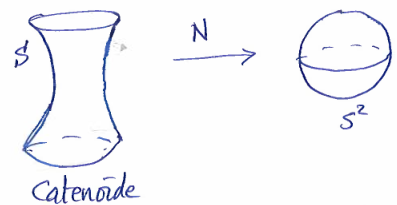
\includegraphics[height=0.8\textheight, width=0.8\textwidth, keepaspectratio]{./Images/catenoide_sphere_14.png}
		\end{center}
	\end{figure}
\end{example}
\subsection{O Grupo Conforme}
\begin{def*}
	Para uma superfície S, o seu \textbf{grupo conforme} é o grupo
	\[
		C_S = \{f:S\rightarrow S:\text{ f é conforme}\}. \; \square
	\]
\end{def*}
O grupo conforme pode ser usado para verificar se duas superfícies diferentes são conformes, pois se os grupos não forem isomorfos, elas não são conformes.
\begin{theorem*}
	Munido da operação de composição de funções, \(C_S\) é um grupo.
\end{theorem*}
\begin{proof*}
	A identidade \(I:S\rightarrow S,\; I(p) = p\) é uma aplicação conforme com \(\lambda_{I} = 1\).

	Além disso, sejam f e g duas funções em \(C_{S}\). A aplicação \(f\circ g:S\stackrel{g}\rightarrow S\stackrel{f}S\) é um difeomorfismo pois f e g são difeomorfismo; daí, temos
	\begin{align*}
		\langle \mathrm{d}(f\circ g)_{p}(w_1), \mathrm{d}(f\circ g)_{p}(w_2) \rangle & = \langle \mathrm{d}f_{g(p)}(\mathrm{d}g_{p}(w_1)), \mathrm{d}f_{g(;)}(\mathrm{d}f_{p}(w_2)) \rangle \\
		                                                                             & = \lambda_f(g(p))\langle \mathrm{d}g_{p}(w_1), \mathrm{d}g_p(w_2) \rangle                            \\
		                                                                             & = \lambda_{f}(g(p))\lambda_{g(p)}\langle w_1, w_2 \rangle                                            \\
		                                                                             & = \lambda_{f\circ g}(p)\langle w_1, w_2 \rangle,
	\end{align*}
	onde \(\lambda_{f\circ g}(p) = \lambda_{f}(g(p))\lambda_{g}(p)\); logo, \(f\circ g\in C_{S}\).

	Seja f um elemento do grupo conforme, tal que a aplicação \(f^{-1}:S\rightarrow S\) é um difeomorfismo. Vamos computar
	\[
		\langle (\mathrm{d}f^{-1})_{q}(w_1), (\mathrm{d}f^{-1})_{q}(w_2)  \rangle, \quad q=f(p).
	\]
	Como f é um difeomorfismo, \(\mathrm{d}f_p:T_pS\rightarrow T_qS\) é um isomorfismo, garantindo a existência de \(v_1,\; v_2\in T_pS\) tais que
	\[
		w_1 = \mathrm{d}f_{p}(v_1) \quad\&\quad w_2 = \mathrm{d}f_p(v_2).
	\]
	Consequentemente,
	\begin{align*}
		\langle (\mathrm{d}f^{-1})_{q}(w_1), (\mathrm{d}f^{-1})_{q}(w_2) \rangle & = \langle \mathrm{d}f_{f(p)}^{-1}(\mathrm{d}f_{p}(v_1)), \mathrm{d}f_{f(p)}^{-1}(\mathrm{d}f_{p}(v_2)) \rangle \\
		                                                                         & =\langle (\mathrm{d}(f^{-1}\circ f))_{p}(v_1), (\mathrm{d}(f^{-1}\circ f))_{p}(v_2)  \rangle                   \\
		                                                                         & = \langle v_1, v_2 \rangle;
	\end{align*}
	porém,
	\[
		\langle w_1, w_2 \rangle =\langle \mathrm{d}f_{p}(v_1), \mathrm{d}f_{p}(v_2) \rangle = \lambda_{f}(p)\langle v_1, v_2 \rangle.
	\]
	Portanto,
	\[
		\langle \mathrm{d}f_{q}^{-1}(w_1), \mathrm{d}f_{q}^{-1}(w_2) \rangle = \frac{1}{\lambda_{f}(f^{-1}(q))} \langle w_1, w_2 \rangle,
	\]
	finalmente levando a \(f^{-1}\in C_{S}\) com \(\displaystyle \lambda_{f^{-1}}(q) = \frac{1}{\lambda_{f}(f^{-1}(q))}\). \qedsymbol
\end{proof*}
\begin{exr}
	Calcule o grupo conforme do plano, da esfera e do plano hiperbólico.
\end{exr}
Suponha que \(f:S\rightarrow \tilde{S}\) é uma aplicação conforme; então, para todo g em \(C_{s}\), a aplicação \(\tilde{g} = f\circ g\circ f^{-1}\in C_{\tilde{S}},\) ou seja, o diagrama abaixo comuta:
\begin{center}
	\begin{tikzpicture}[
			observed/.style = {rectangle, thick, text centered, draw, text width = 6em},
			latent/.style = {ellipse, thick, draw, text centered, text width = 6em},
			error/.style ={circle, thick, draw, text centered},
			confounding/.style = {rectangle, thick, text centered, draw, text width = 6em, minimum width = 5.5in},
			outcome/.style = {rectangle, thick, draw, text centered, minimum height = 3.5in, text width = 6em},
		]
		\node(TL) at (-1,1){S};
		\node(BL) at (-1,-1){S};
		\node(TR) at (1,1){\(\tilde{S}\)};
		\node(BR) at (1,-1){\(\tilde{S}\)};

		\draw[Arrow](TL)--node[midway, above] {f}(TR);
		\draw[Arrow](BL)--node[midway, below] {f}(BR);
		\draw[Arrow](TL)--node[midway, left] {g}(BL);
		\draw[Arrow](TR)--node[midway, right] {\(\tilde{g}\)}(BR);

	\end{tikzpicture}
\end{center}
A aplicação \(J_{f}:C_{s}\rightarrow C_{\tilde{S}}\) com \(J_{f}(g) = f\circ g\circ f^{-1}\) é um isomorfismo! Consequentemente, se S e \(\tilde{S}\) são conformes, podemos concluir que seus grupos conformes serão isomorfos; por outro lado, caso \(C_S\) e \(C_{\tilde{S}}\) não são isomorfos, então S e \(\tilde{S}\) não serão conformes.
\begin{theorem*}
	Duas superfícies regulares quaisquer são localmente conformes.
\end{theorem*}
\begin{proof*}
	Seja S uma superfície regular; então, para cada ponto p em S, existe uma parametrização local
	\[
		\underline{x}:U\subseteq \mathbb{R}^{2}\rightarrow S,
	\]
	com \(p\in \underline{x}(U)\), tal que \(E = \lambda (u, v) > 0,\; F=0,\; G = \lambda (u,v)\), conhecida como \textbf{parametrização isométrica de S}.
	Portanto, S é localmente conforme ao plano. \qedsymbol
\end{proof*}

\end{document}

